\documentclass{standalone}
\usepackage{graphicx}	
\usepackage{amssymb, amsmath}
\usepackage{color}

\usepackage{tikz}
\usetikzlibrary{arrows.meta, backgrounds, math}
\usepackage{pgfmath}

\definecolor{light}{RGB}{220, 188, 188}
\definecolor{mid}{RGB}{185, 124, 124}
\definecolor{dark}{RGB}{143, 39, 39}
\definecolor{highlight}{RGB}{180, 31, 180}
\definecolor{light_teal}{RGB}{107, 142, 142}
\definecolor{mid_teal}{RGB}{72, 117, 117}
\definecolor{dark_teal}{RGB}{29, 79, 79}
\definecolor{gray10}{gray}{0.1}
\definecolor{gray20}{gray}{0.2}
\definecolor{gray30}{gray}{0.3}
\definecolor{gray40}{gray}{0.4}
\definecolor{gray60}{gray}{0.6}
\definecolor{gray70}{gray}{0.7}
\definecolor{gray80}{gray}{0.8}
\definecolor{gray90}{gray}{0.9}
\definecolor{gray95}{gray}{0.95}

\begin{document}

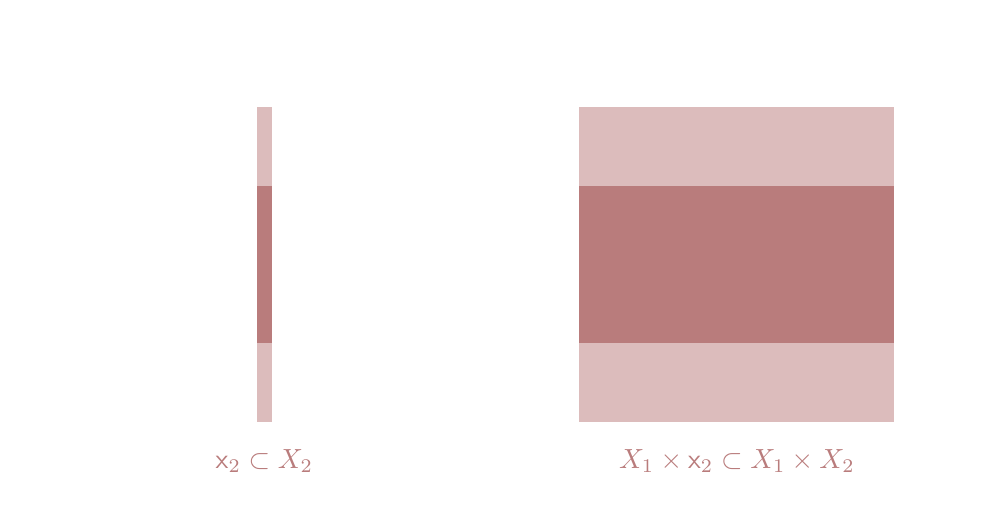
\begin{tikzpicture}[scale=1.0]
  
  \begin{scope}[shift={(0, -6)}]
    \draw[white] (-3, -3) rectangle (3, 3);
    
    \fill[light] (-0.1, -2) rectangle (0.1, 2);
    
    \fill[mid] (-0.1, -1) rectangle (0.1, 1);
    
    \node[mid] at (0, -2.5) 
      { $\mathsf{x}_{2} \subset X_{2}$ };
  \end{scope}
  
  \begin{scope}[shift={(6, -6)}]
    \draw[white] (-3, -3) rectangle (3, 3);
    
    \fill[light] (-2, -2) rectangle (2, 2);
    
    \fill[mid] (-2, -1) rectangle (2, 1);
      
    \node[mid] at (0, -2.5) 
      { $X_{1} \times \mathsf{x}_{2} \subset X_{1} \times X_{2}$ };
      
  \end{scope}
  
\end{tikzpicture}

\end{document}  